
\documentclass[11pt, a4paper]{article}
\usepackage[utf8]{inputenc}
\usepackage[T1]{fontenc}
\usepackage{geometry}
\usepackage{xcolor}
\usepackage{hyperref}
\usepackage{enumitem}
\usepackage{titlesec}
\usepackage{mathpazo}
\usepackage{graphicx}
\usepackage{float}


\geometry{margin=25mm}

% Define colors
\definecolor{hecblue}{RGB}{0, 51, 102}
\definecolor{lightgrey}{RGB}{245, 245, 245}

% Section styling
\titleformat{\section}{\large\bfseries\color{hecblue}}{\thesection}{1em}{}[{\titlerule[0.5pt]}]
\titleformat{\subsection}{\normalsize\bfseries\color{hecblue}}{\thesubsection}{1em}{}

\title{\textbf{HEC-RAS 2D Dynamic River Simulation Guide}}
\author{Technical Documentation}
\date{\today}

\begin{document}

\maketitle

\section{Introduction}
This document outlines the workflow for conducting a 2D unsteady flow (dynamic) simulation in HEC-RAS using a topobathymetric GeoTIFF and known water surface elevations (heads).

\section{Part 1: Setting Up the Terrain}
Before performing hydraulic calculations, HEC-RAS requires a Digital Elevation Model (DEM) in a specific format (.hdf).

\subsection{Open HEC-RAS:} 
Create a new project.

\begin{figure}[H]
\centering

\includegraphics[width=0.80\textwidth]{Jpg/Figure1.png}
\caption{Create project}
%\label{fig:sample1}
\end{figure}

But be careful of the unit system
\begin{figure}[H]
\centering

\includegraphics[width=0.80\textwidth]{Jpg/Figure2.png}
\caption{Warning over the unit system}
%\label{fig:sample1}
\end{figure}

Before importing shapefile its time to change the unit system of the project. Go to Options > Unit System (US Customary or System International).Select System International (SI): Meters, kilometers, etc.

\begin{figure}[H]
\centering
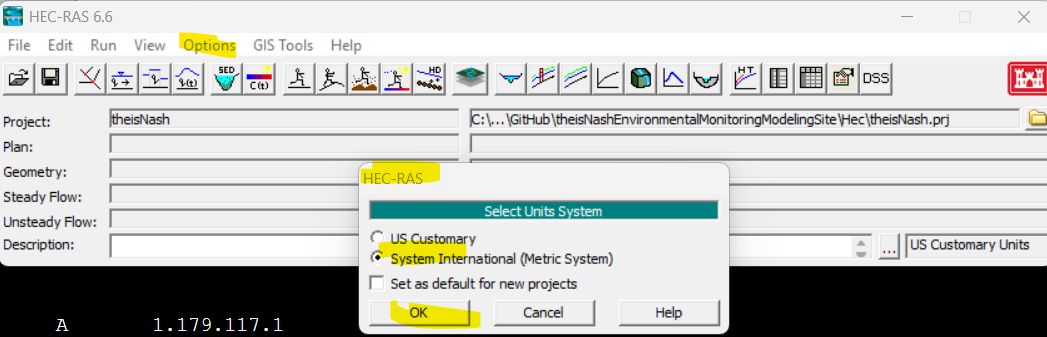
\includegraphics[width=0.80\textwidth]{Jpg/Figure10a.png}
\caption{Select Units System}
%\label{fig:sample1}
\end{figure}

\newpage

\subsection{RAS Mapper:} 
Open the RAS Mapper tool.
\begin{figure}[H]
\centering

\includegraphics[width=0.80\textwidth]{Jpg/Figure3.png}
\caption{Ras Mapper tool}
%\label{fig:sample1}
\end{figure}

\subsubsection{Coordinate System:} 
Go to \textit{Project > Set Projection}. Select a Projection file (.prj) that matches your GeoTIFF's coordinate system.

\begin{figure}[H]
\centering

\includegraphics[width=0.80\textwidth]{Jpg/Figure4.png}
\caption{Set projection}
%\label{fig:sample1}
\end{figure}

\subsubsection{Create Terrain:} 
Right-click on \textit{Terrains} and select \textit{Create New RAS Terrain}. 

\begin{figure}[H]
\centering

\includegraphics[width=0.80\textwidth]{Jpg/Figure5.png}
\caption{Create New RAS Terrain}
%\label{fig:sample1}
\end{figure}

Add your topobathymetric \texttt{.tif} file. This will convert the GeoTIFF into a HEC-RAS Terrain layer.

\begin{figure}[H]
\centering

\includegraphics[width=0.80\textwidth]{Jpg/Figure6.png}
\caption{Add your tif file}
%\label{fig:sample1}
\end{figure}

\begin{figure}[H]
\centering

\includegraphics[width=0.80\textwidth]{Jpg/Figure7.png}
\caption{Hdf creation}
%\label{fig:sample1}
\end{figure}

\newpage

\section{Part 2: Defining the 2D Flow Area}

\subsubsection{Create Geometry:} 
In RAS Mapper, right-click \textit{Geometries} and select \textit{Add New Geometry}.


\begin{figure}[H]
\centering

\includegraphics[width=0.80\textwidth]{Jpg/Figure8.png}
\caption{Add New Geometry}
%\label{fig:sample1}
\end{figure}

\begin{figure}[H]
\centering

\includegraphics[width=0.80\textwidth]{Jpg/Figure9.png}
\caption{New Geometry Data}
%\label{fig:sample1}
\end{figure}

\begin{figure}[H]
\centering

\includegraphics[width=0.80\textwidth]{Jpg/Figure10.png}
\caption{Manage Layer Associations}
%\label{fig:sample1}
\end{figure}


\subsubsection{Import the Shapefile into a Layer} 
You cannot simply "open" a shapefile as a geometry; you must import its features into the specific HEC-RAS layer (like the 2D Flow Area / Perimeter).

\begin{figure}[H]
\centering

\includegraphics[width=0.80\textwidth]{Jpg/Figure11.png}
\caption{Edit geometry}
%\label{fig:sample1}
\end{figure}

\subsubsection{Create Geometry:} 
Right-click on the specific sub-layer you want to populate (e.g., 2D Flow Areas / Perimeters).

\begin{figure}[H]
\centering

\includegraphics[width=0.80\textwidth]{Jpg/Figure12.png}
\caption{Feature Import}
%\label{fig:sample1}
\end{figure}

Right-click the 2D area polygon and select \textit{Edit 2D Flow Area Properties}.

\begin{figure}[H]
\centering

\includegraphics[width=0.80\textwidth]{Jpg/Figure13.png}
\caption{Edit 2D Flow Area Properties}
%\label{fig:sample1}
\end{figure}

Define your cell size (e.g., 2m x 2m). Click \textit{Generate Computation Points}.

\begin{figure}[H]
\centering
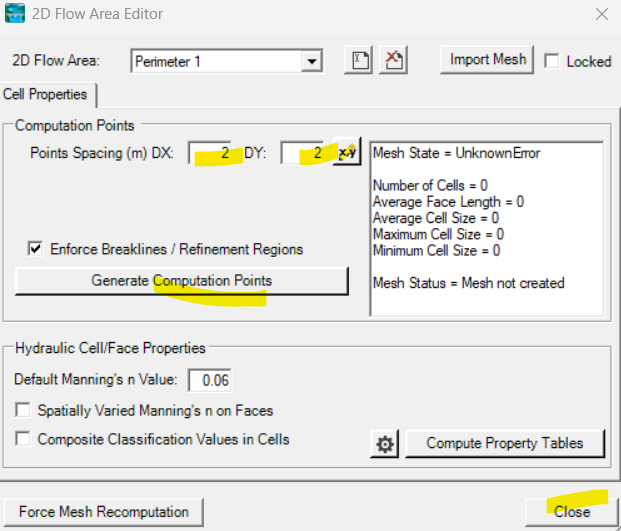
\includegraphics[width=0.80\textwidth]{Jpg/Figure14.png}
\caption{Edit 2D Flow Area Properties}
%\label{fig:sample1}
\end{figure}

\newpage 

\section{Part 3: Boundary Conditions}
Since you have "heads" (Water Surface Elevations - WSE), you will use these as boundary conditions.

\subsection{Boundary Condition Lines} 
In RAS Mapper, select the \textit{Boundary Condition Lines} layer under your Geometry.

\begin{figure}[H]
\centering
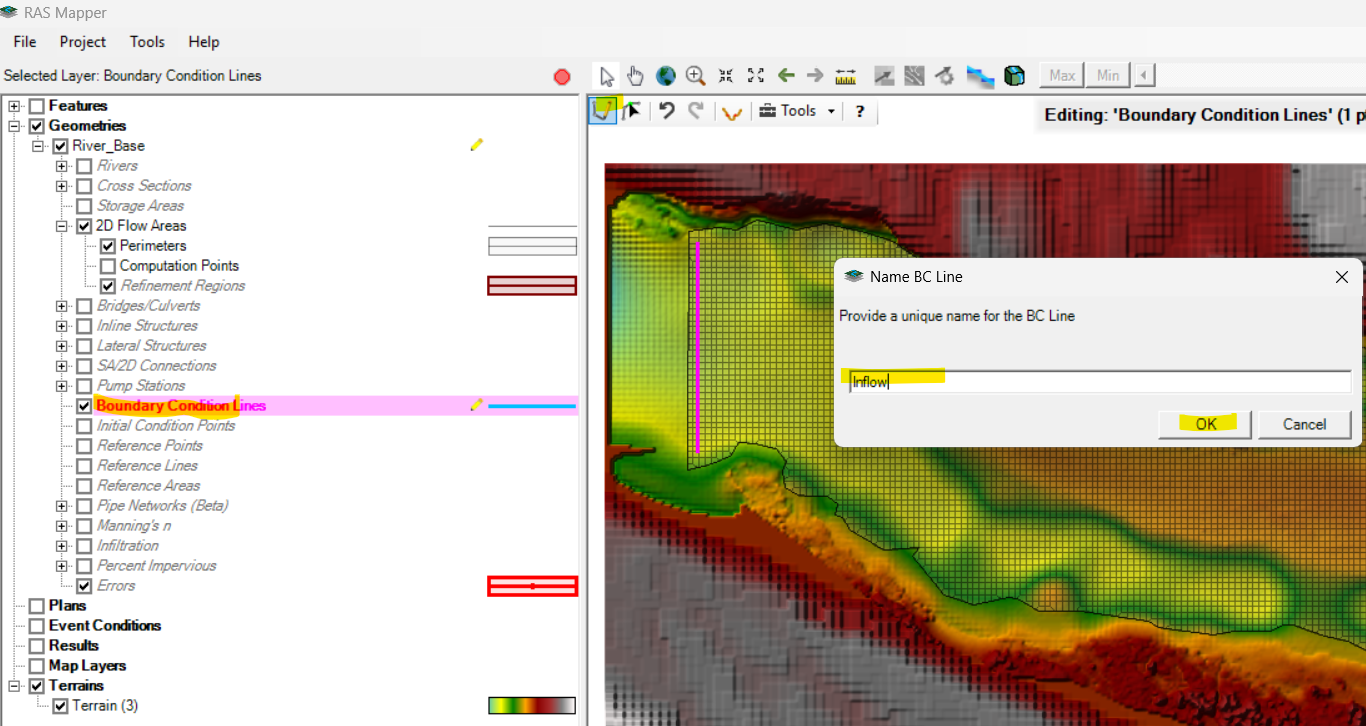
\includegraphics[width=0.80\textwidth]{Jpg/Figure15.png}
\caption{Name BC Line - Inflow}
%\label{fig:sample1}
\end{figure}

The outflow boundary condition has to be outside the model on the downstream direction.

\begin{figure}[H]
\centering
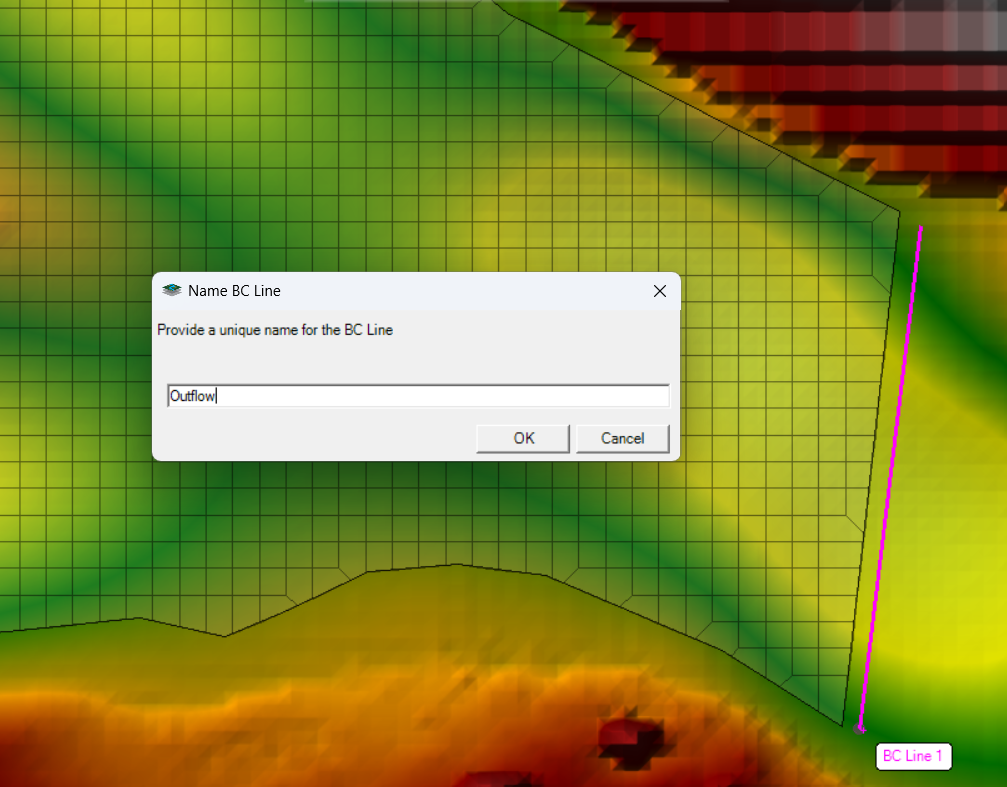
\includegraphics[width=0.80\textwidth]{Jpg/Figure16.png}
\caption{Name BC Line - Outflow}
%\label{fig:sample1}
\end{figure}

\newpage

Close the editing mode for the recomputation of the line conectivity

\begin{figure}[H]
\centering
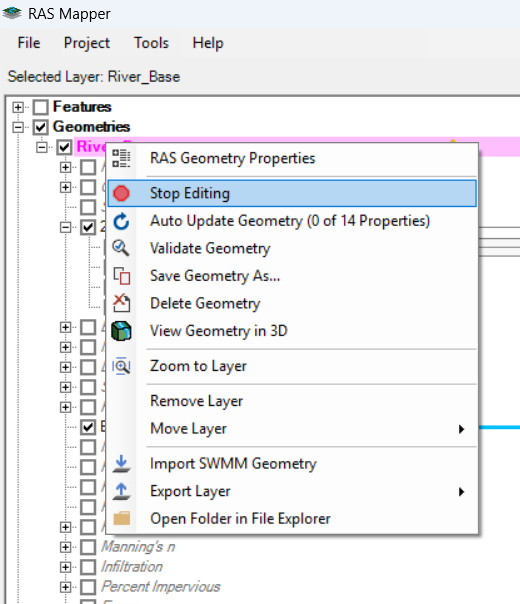
\includegraphics[width=0.80\textwidth]{Jpg/Figure16a.png}
\caption{Close editing mode}
%\label{fig:sample1}
\end{figure}

Open attribute table of the boundary condition lines. Check that Inflow is set as Internal and Outflow is set as External.

\begin{figure}[H]
\centering
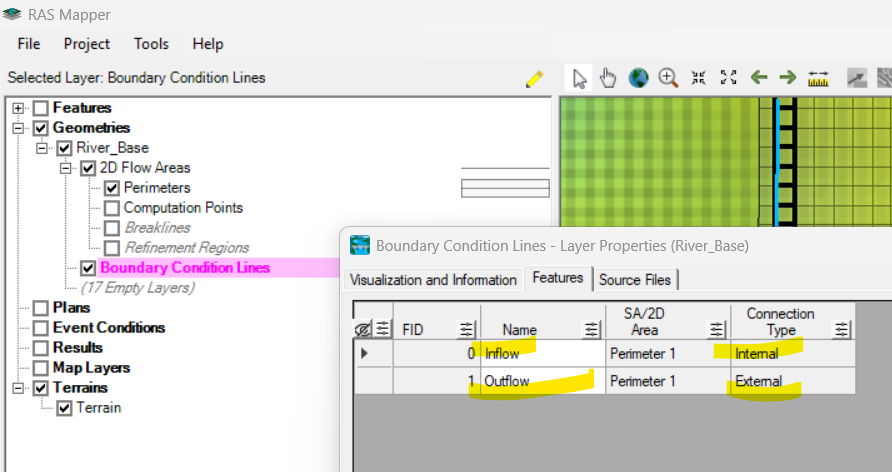
\includegraphics[width=0.80\textwidth]{Jpg/Figure16b.png}
\caption{Layer Properties of Boundary Conditions}
%\label{fig:sample1}
\end{figure}

You can save your RAS Mapper project just in case.

\newpage



\section{Set up geometry in the HEC RAS project}

In HecRas open Edit / Geometric Data

Open the saved geometry. The geometry should appear in the Geometric Data window and the path should appear on the HEC RAS project.

\begin{figure}[H]
\centering
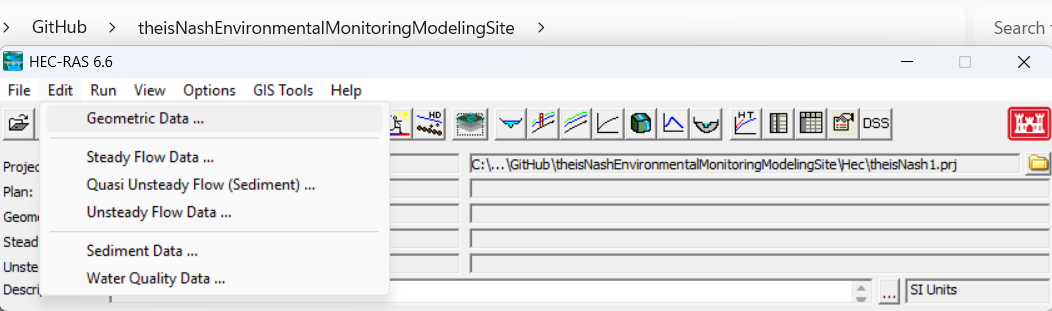
\includegraphics[width=0.80\textwidth]{Jpg/Figure17.png}
\caption{Edit Geometric Data}
%\label{fig:sample1}
\end{figure}

We open the saved geometric data to check that is ok and also to ensure that the HEC project recognizes this geometry.

\begin{figure}[H]
\centering
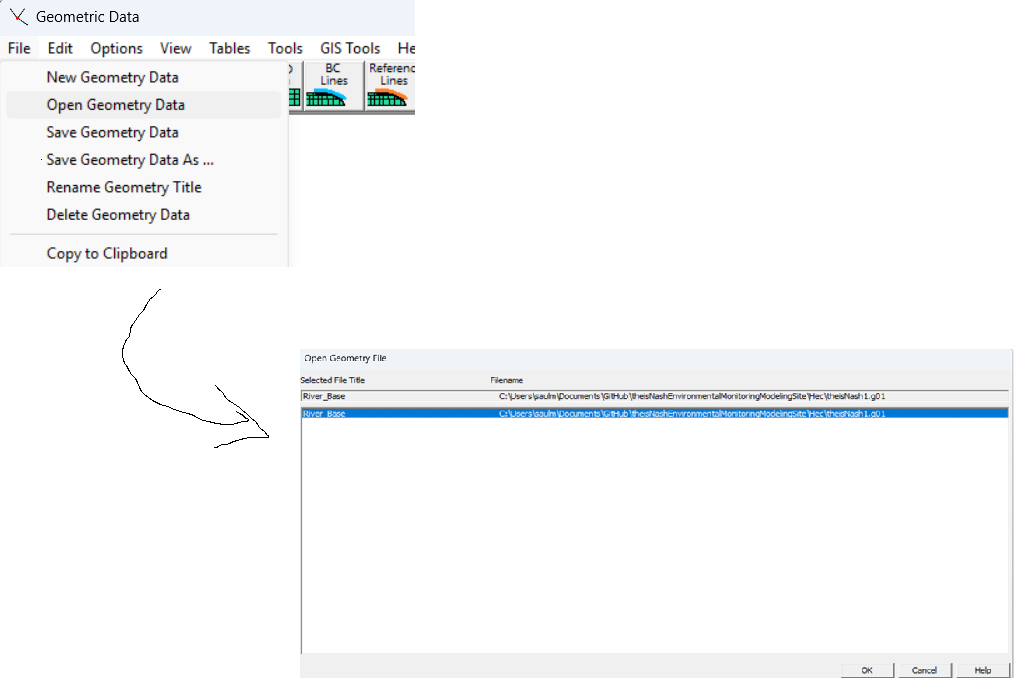
\includegraphics[width=0.80\textwidth]{Jpg/Figure18.png}
\caption{Open the saved geometry}
%\label{fig:sample1}
\end{figure}

\newpage 

Imported geometry in the HEC project.

\begin{figure}[H]
\centering
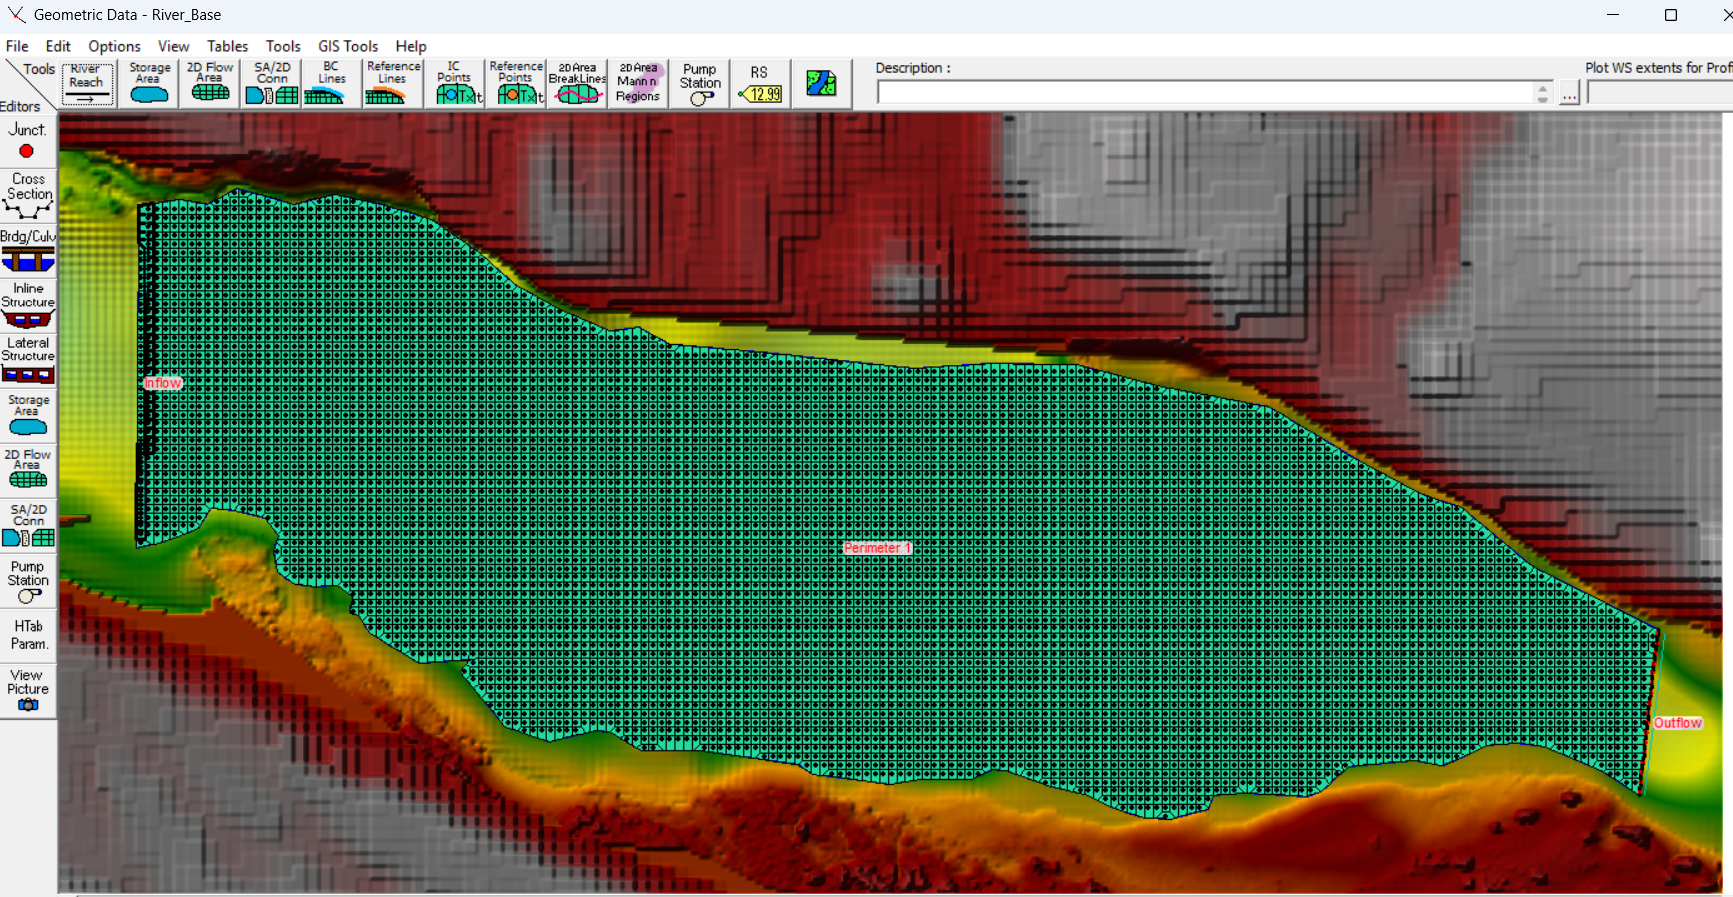
\includegraphics[width=0.80\textwidth]{Jpg/Figure19.png}
\caption{Imported geometry in the HEC project}
%\label{fig:sample1}
\end{figure}

Close the Geometric Data window and you will see that the RiverBase geometry is part of the HEC RAS project.

\begin{figure}[H]
\centering
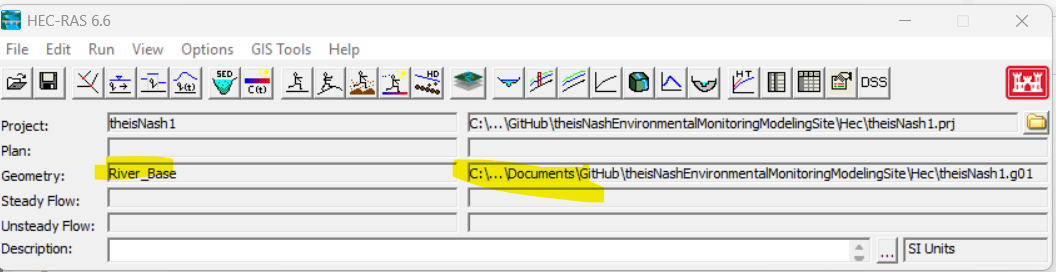
\includegraphics[width=0.80\textwidth]{Jpg/Figure20.png}
\caption{HEC RAS project with the geometry}
%\label{fig:sample1}
\end{figure}

\newpage

\subsection{Define Unsteady Flow Data}

Press the view/edit unsteady flow data bottom. You will see the following.

\begin{figure}[H]
\centering
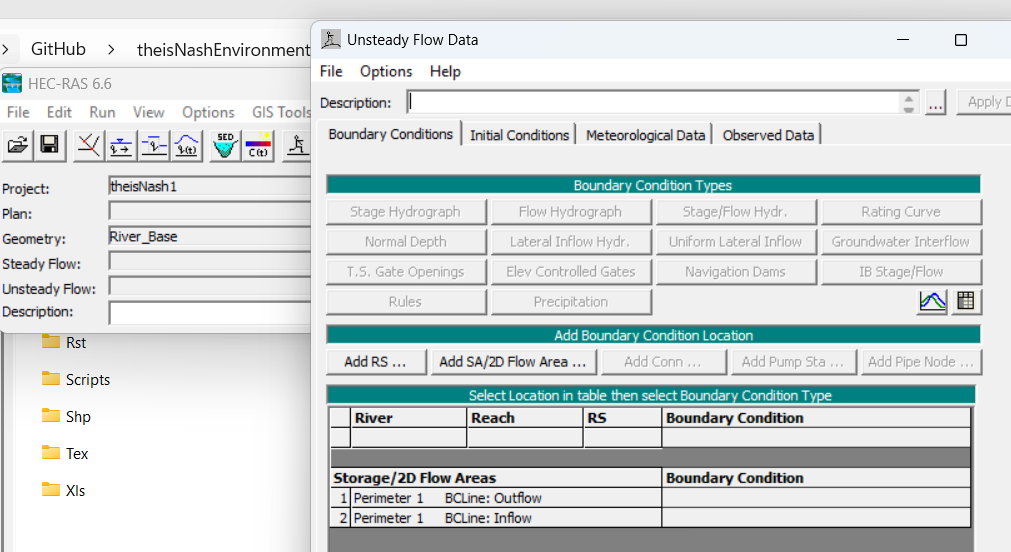
\includegraphics[width=0.80\textwidth]{Jpg/Figure21.png}
\caption{Unsteady Flow Data}
%\label{fig:sample1}
\end{figure}

For the Inflow boundary condition we are going to set up a flow hydrograph. Flow data is imported from a DSS file. Check the plot to see if imported correctly.

\begin{figure}[H]
\centering
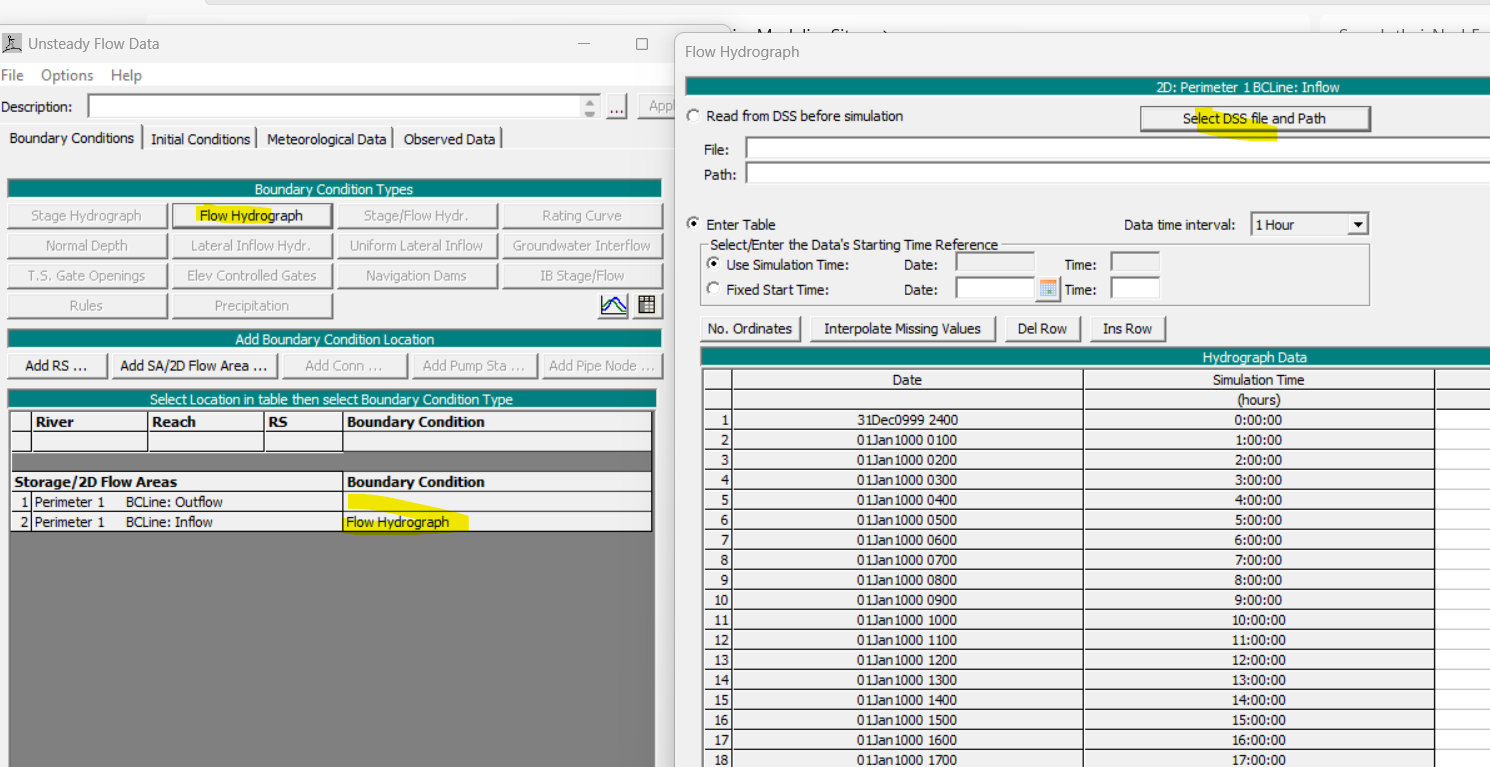
\includegraphics[width=0.80\textwidth]{Jpg/Figure22.png}
\caption{Flow of Inflow Boundary Condition}
%\label{fig:sample1}
\end{figure}

\newpage

\begin{figure}[H]
\centering
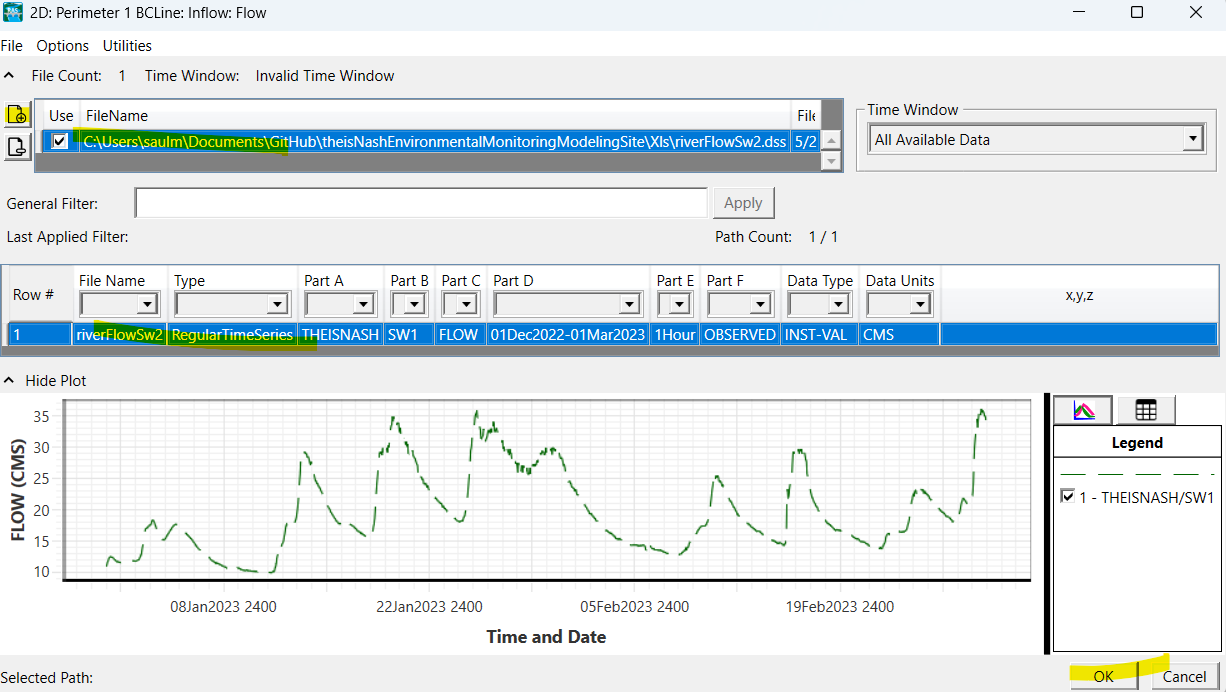
\includegraphics[width=0.80\textwidth]{Jpg/Figure23.png}
\caption{Flow of Inflow Boundary Condition}
%\label{fig:sample1}
\end{figure}

The Outflow BC will be set as Normal Depth meaning that all water that reaches the bc will leave the model.

\begin{figure}[H]
\centering
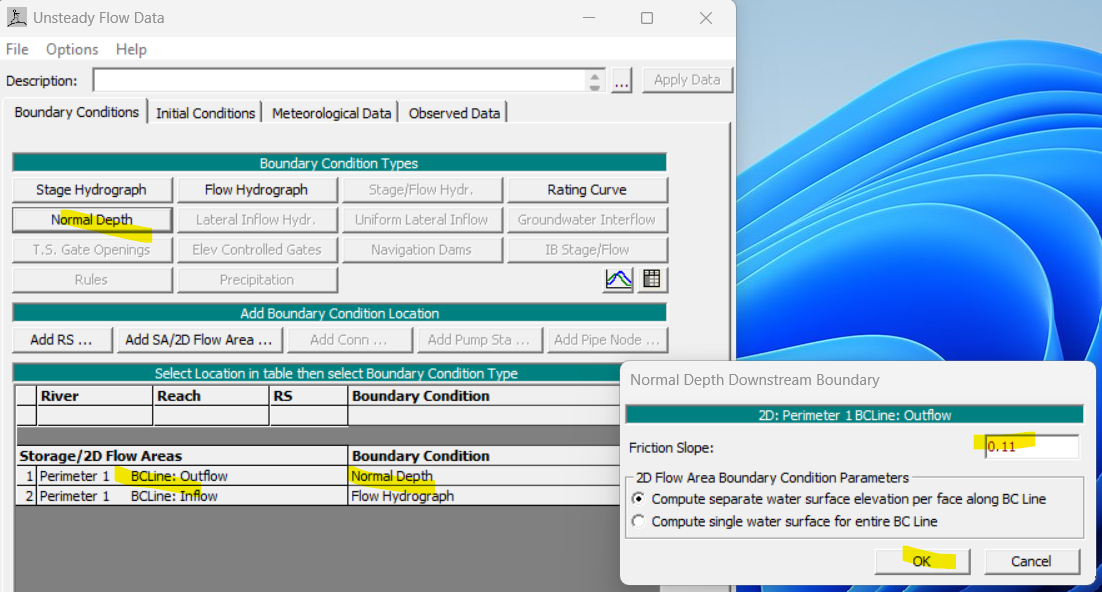
\includegraphics[width=0.80\textwidth]{Jpg/Figure24.png}
\caption{Outflow BC configuration}
%\label{fig:sample1}
\end{figure}

\newpage

Save the unsteady flow data as Unsteady1 and close. After check that the data is imported into the project.

\begin{figure}[H]
\centering
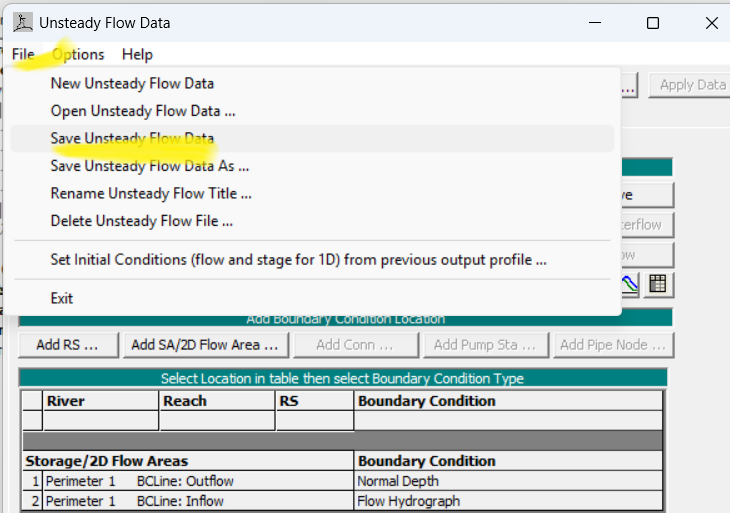
\includegraphics[width=0.80\textwidth]{Jpg/Figure25.png}
\caption{Save the unsteady flow data}
%\label{fig:sample1}
\end{figure}

\newpage

\subsection{Unsteady Flow Analysis}

Now its time to create a plan that compiles the geometry and flow. On Unsteady Flow Analysis fill the following.
For the Computation Interval we have to take into account Courant. The cross section area is around 40 m2 and flow is around 16m3, so the average velocity is 0.4m/s. If the cell size is 2 meters that means that a particle of water will take 5 seconds to cross it. Therefore the computation interval has to be smaller, we will set up to 4 seconds, otherwise we are going to have unconvergences and wrong simulations.

\begin{figure}[H]
\centering
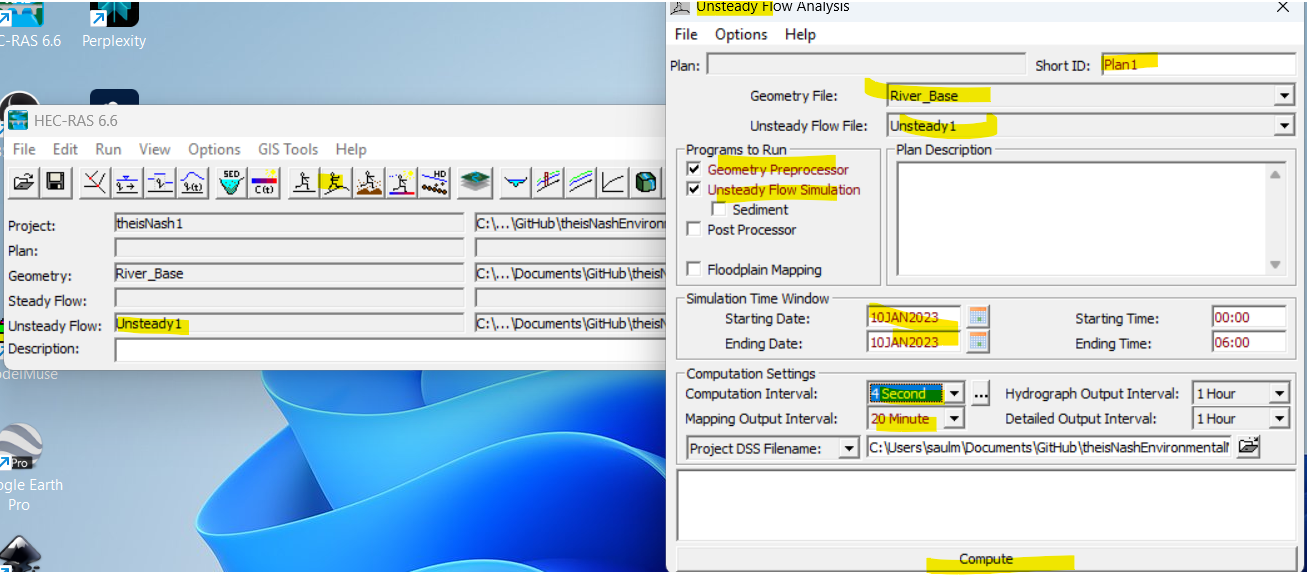
\includegraphics[width=0.80\textwidth]{Jpg/Figure26.png}
\caption{Unsteady flow analysis}
%\label{fig:sample1}
\end{figure}

\begin{figure}[H]
\centering
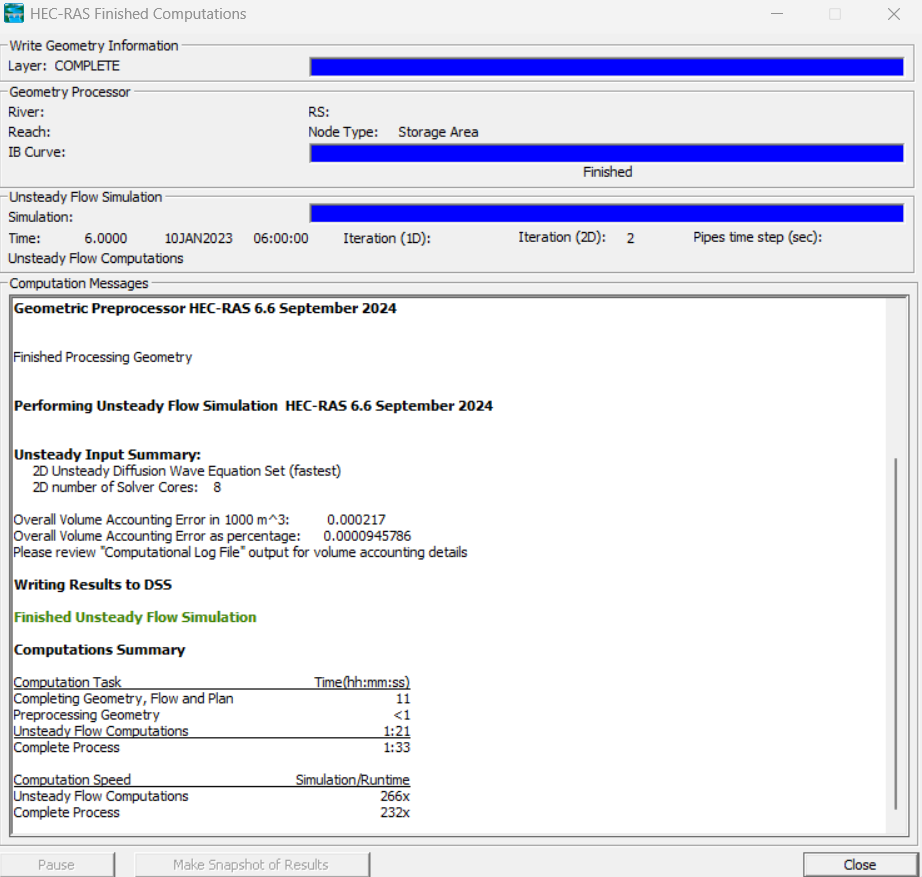
\includegraphics[width=0.80\textwidth]{Jpg/Figure27.png}
\caption{End of the unsteady flow simulations}
%\label{fig:sample1}
\end{figure}

\newpage

\subsection{Result analysis}

Save the plan and open RAS Mapper. Results are already available.

\begin{figure}[H]
\centering
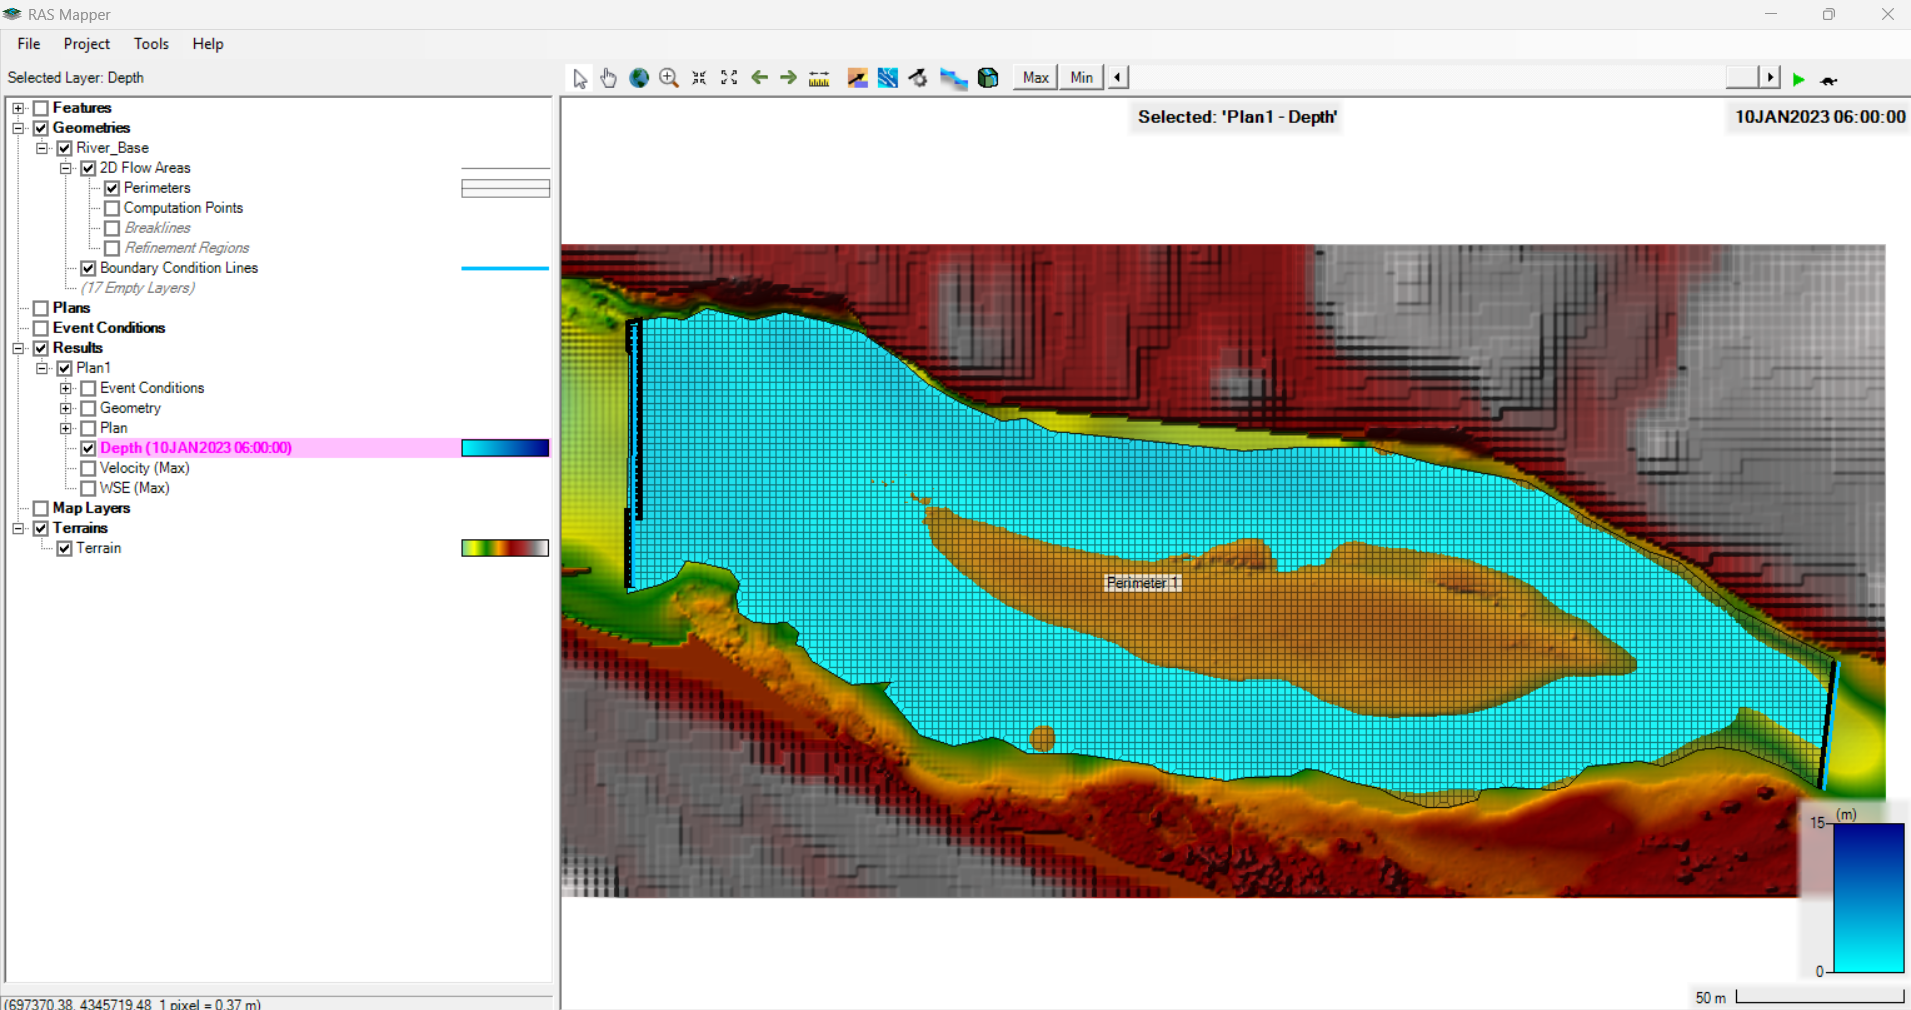
\includegraphics[width=0.80\textwidth]{Jpg/Figure28.png}
\caption{Depth visualization}
%\label{fig:sample1}
\end{figure}

\begin{figure}[H]
\centering
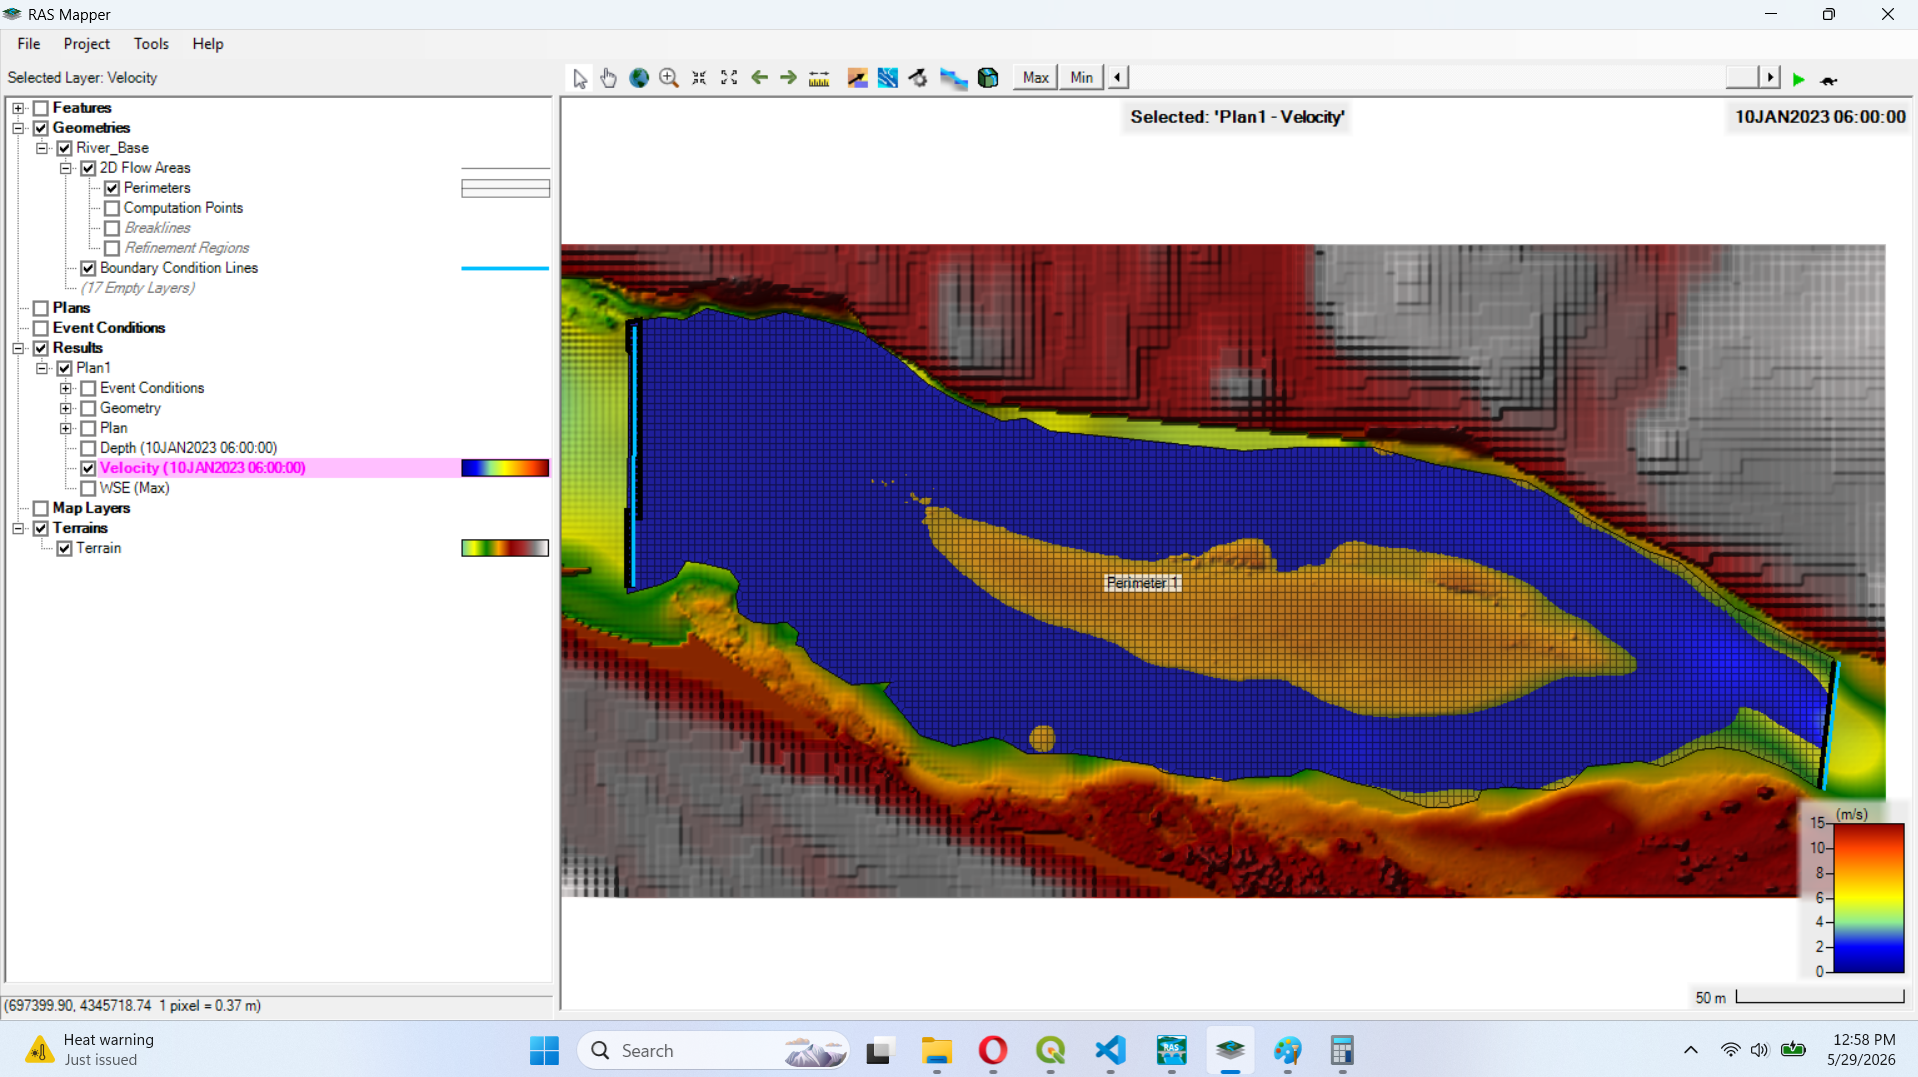
\includegraphics[width=0.80\textwidth]{Jpg/Figure29.png}
\caption{Velocity visualization}
%\label{fig:sample1}
\end{figure}

\newpage

\begin{figure}[H]
\centering
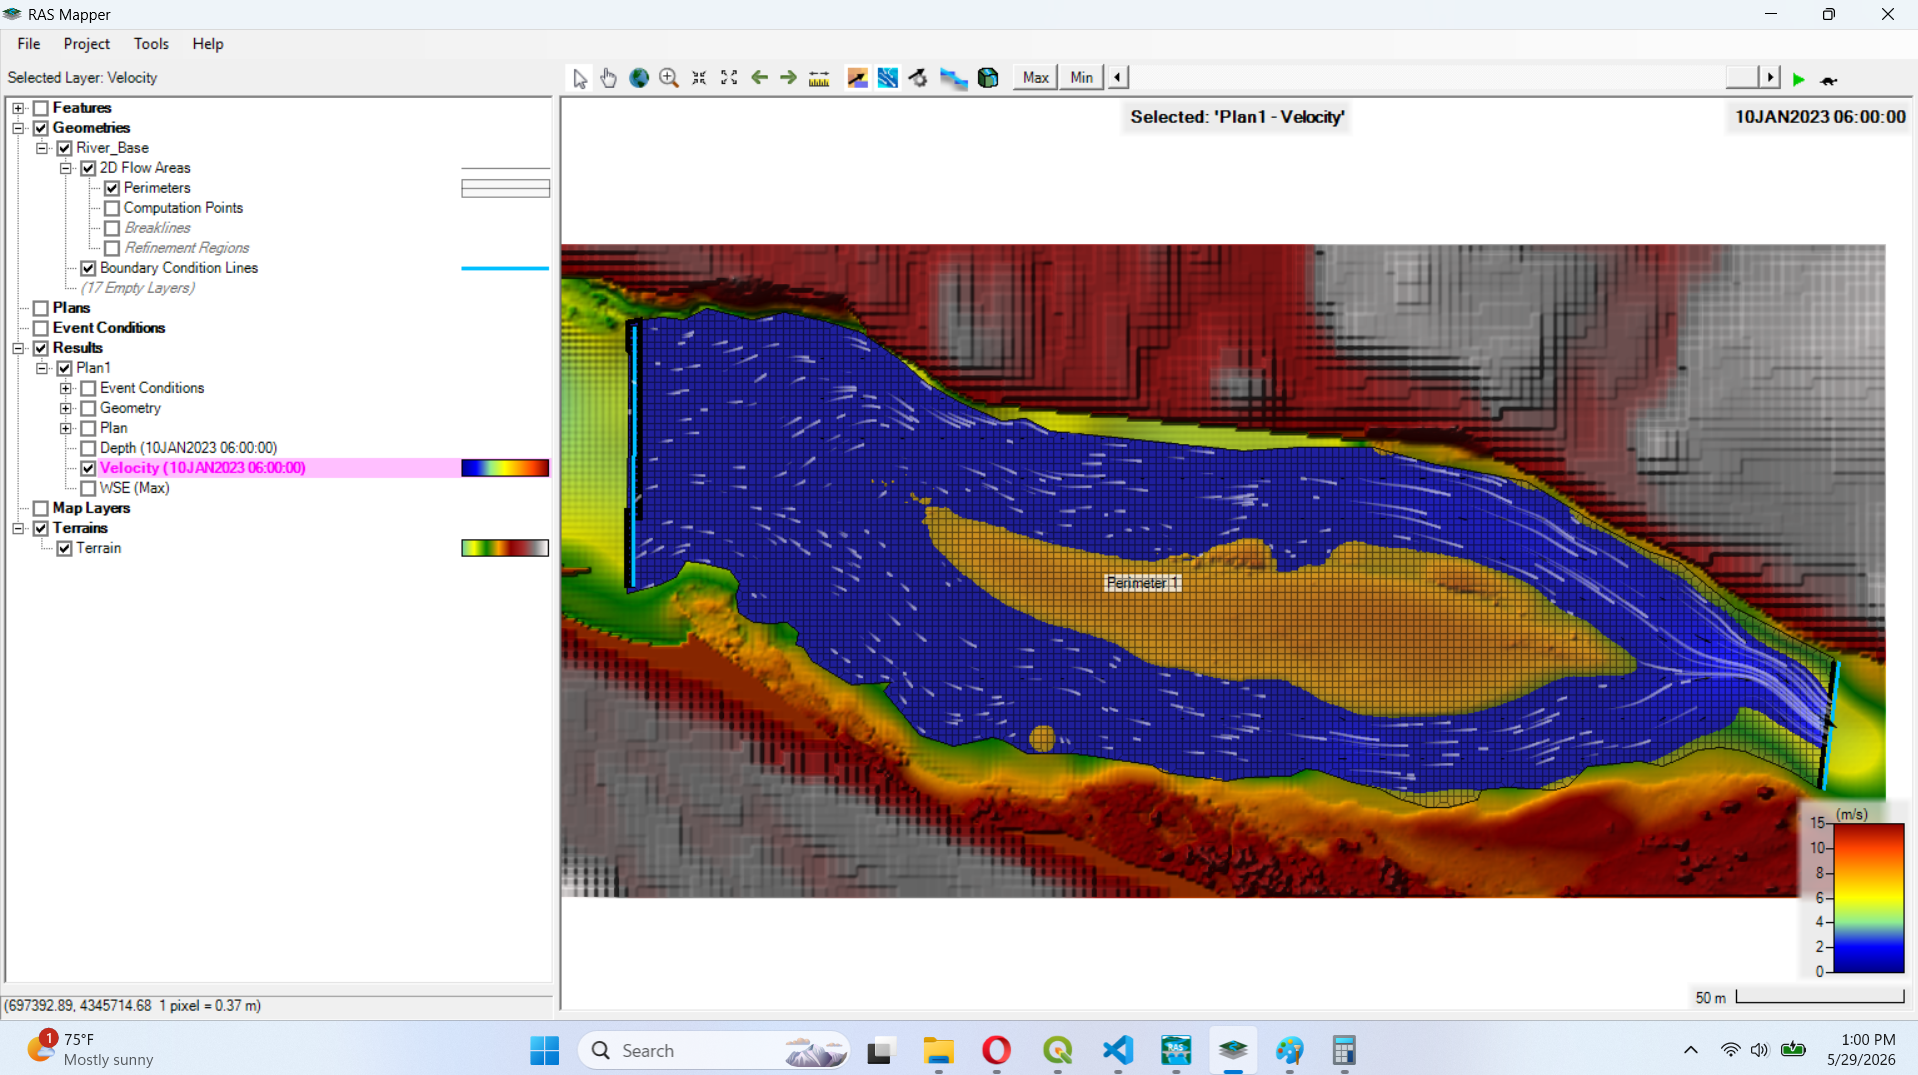
\includegraphics[width=0.80\textwidth]{Jpg/Figure30.png}
\caption{Particle tracking}
%\label{fig:sample1}
\end{figure}

\end{document}
